\documentclass[12pt,a4j,fleqn]{jsarticle}
\usepackage{geometry}
\usepackage{amsmath}
\usepackage{amssymb}
\usepackage{txfonts}
\usepackage{bm}
\usepackage[dvipdfmx]{graphicx}
\usepackage{booktabs}
\geometry{top=20truemm,bottom=15truemm,left=25truemm,right=10truemm}
\linespread{0.97}  % 1 ページ 40 行
\renewcommand{\figurename}{Fig.~}
\renewcommand{\tablename}{Table~}
\setlength{\mathindent}{2em}
\pagestyle{empty}
\begin{document}
\begin{center}
\textsf{\textgt{\Large IGA-重合パッチ法(S-IGA)の基底関数の高次化に関する研究}}
\end{center}
\vspace{\baselineskip}
\begin{flushleft}
[岡田研究室]
\end{flushleft}
\vspace{-2\baselineskip}
\begin{flushright}
7518074 土山 雄飛
\end{flushright}

有限要素法解析(Finite Element Method, FEM)では,解析モデルの設計が解析全体の約$80\ \%$を占めていると見積もられている.
近年では,解析モデルの生成を短縮するためにメッシュフリー法が研究されており,
その一つにCADの幾何学表現である非一様有理Bスプライン(Non-Uniform Rational B-Spline, NURBS)を
基底関数としたアイソジオメトリック解析(Isogeometric Analysis, IGA)がある.
また,FEM解析の柔軟なモデリングと高精度化が可能となるマルチスケール解析である重合メッシュ法(S-version Finite Element Method, S-FEM)を
IGA解析に応用した手法である重合パッチ法(S-version Isogeometric Analysis Method, S-IGA)が提案されている.

本研究では,IGA解析と重合パッチ法解析における基底関数の次数を高次化した解析例を示し,解析精度を検証した.
IGA解析では,図~\ref{fig:1}に示すように同自由度では2次より3次の基底関数の方が高精度となった.
重合パッチ法解析では,基底関数の次数の組はグローバルパッチとローカルパッチで共に3次とした場合が最も高精度となり,
図~\ref{fig:2},図~\ref{fig:3}に示すように3次の基底関数を用いた方がより滑らかな結果の分布を示した.
また,グローバルパッチの要素サイズに対するローカルパッチの全体サイズの比を2.5倍から4倍の間に設定すると解析精度が低下する現象を
防ぐことができることが確認された.

\begin{figure}[htbp]
  \centering
  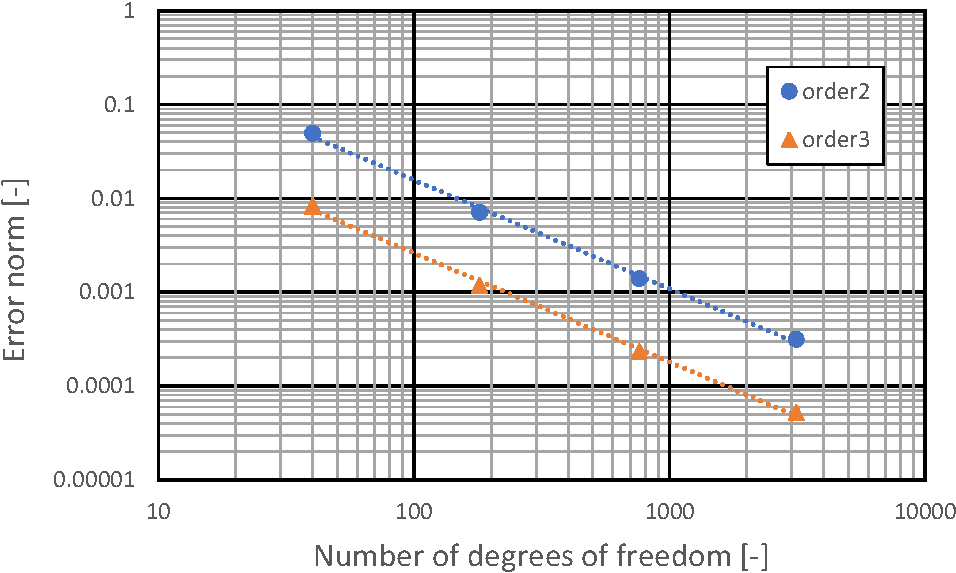
\includegraphics[keepaspectratio, scale = 0.415]
  {fig/ER01-crop.pdf}
  \caption{Error norm of $\sigma_{rr}$ in IGA analysis}
  \label{fig:1}
\end{figure}

\begin{figure}[hbtp]
  \begin{tabular}{cc}
    \begin{minipage}[t]{0.45\hsize}
      \centering
      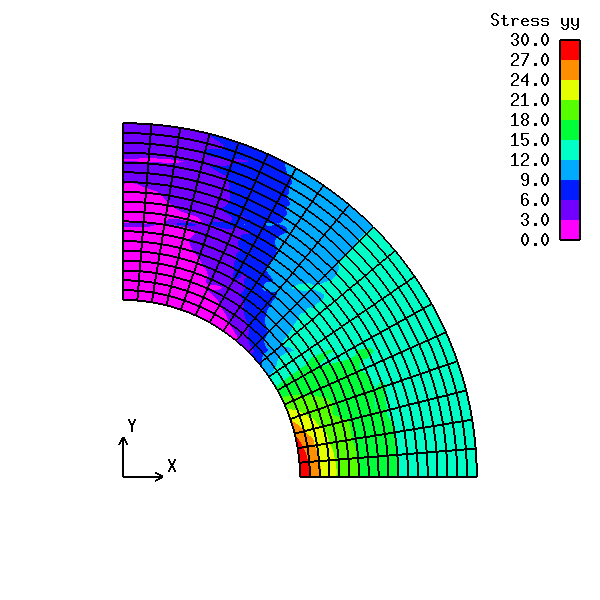
\includegraphics[keepaspectratio, scale=0.18]
      {fig/2.png}
      \caption{Stress in $y$ direction on Local patch in the S-IGA analysis (second-order, Global patch $30\times 30$, Local patch $20\times 20$)}
      \label{fig:2}
    \end{minipage} &
    \begin{minipage}[t]{0.45\hsize}
      \centering
      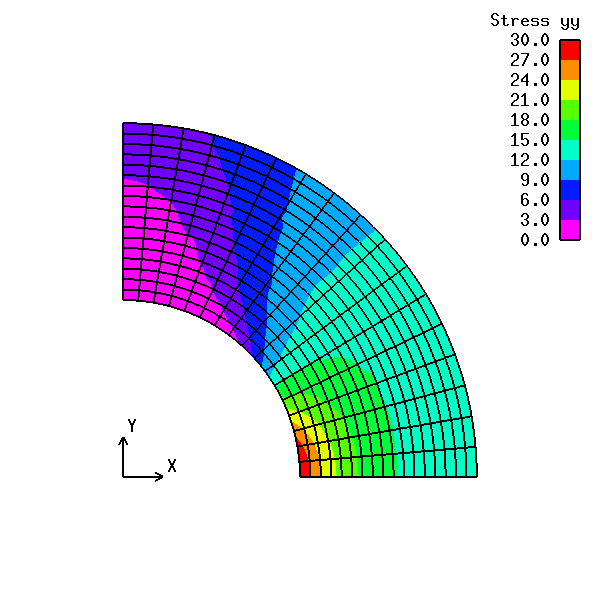
\includegraphics[keepaspectratio, scale=0.18]
      {fig/3.png}
      \caption{Stress in $y$ direction on Local patch in the S-IGA analysis (third-order, Global patch $30\times 30$, Local patch $20\times 20$)}
      \label{fig:3}
    \end{minipage}
  \end{tabular}
\end{figure}

\clearpage
\begin{center}
\textsf{\textgt{\Large Study on higher order of basis functions for S-version Isogeometric Analysis Method}}
\end{center}
\vspace{\baselineskip}
\begin{flushleft}
[Okada Group]
\end{flushleft}
\vspace{-2\baselineskip}
\begin{flushright}
7518074 Yuhi TSUCHIYAMA
\end{flushright}
In Finite Element Method (FEM), it is estimated that
the design of the analytical model accounts for about $80\ \%$ of the total analysis.
%
In recent years, Meshfree method have been studied in order to shorten the generation of analytical models.
%
One of them is Isogeometric Analysis (IGA),
which uses Non-Uniform Rational B-Spline (NURBS),
a geometric representation of CAD,
as basis functions.
%
In addition, the S-version Finite Element Method (S-FEM),
which is a multi-scale analysis that enables flexible modeling and high accuracy of FEM analysis,
has been proposed to be applied to IGA analysis, S-version Isogeometric Analysis Method (S-IGA).
%
In this study, examples of IGA analysis and S-IGA analysis
with higher order of basis functions are presented to verify the accuracy of the analysis.
%
In the IGA analysis,
the third-order basis functions were more accurate than the second-order basis functions for the same degrees of freedom.
%
In the S-IGA analysis, the highest accuracy was obtained when the order of basis functions was set to the third-order for both the Global and Local patches.
%
The distribution of results was smoother when the third-order basis functions were used.
%
It was also confirmed that setting the ratio of the overall size of the Local patch to the element size of the Global patch
between 2.5 and 4 times prevented the phenomenon of reduced analysis accuracy.
\end{document}